\documentclass[a4paper]{article}

\usepackage{geometry}
\usepackage{indentfirst}
\usepackage{amsmath,amssymb}
\usepackage{amsthm}
\DeclareMathOperator*{\argmax}{arg\,max}
\usepackage{amsthm}
\usepackage{bm}
\usepackage{bbm}
\usepackage{graphicx}
\usepackage{float}
\usepackage{color}
\usepackage{algorithm}
\usepackage{algorithmic}
%\renewcommand{\algorithmicrequire}{\textbf{Initialization:}}
%\renewcommand{\algorithmicensure}{\textbf{Inference:}}

\geometry{left=3cm,right=3cm,top=3.75cm,bottom=3.75cm}
\setlength{\parindent}{0em}
\setlength{\parskip}{1em}


\begin{document}

\newtheorem{thm}{Theorem}
\newtheorem*{thm*}{Theorem}
\newtheorem{lem}{Lemma}
\newtheorem{cla}{Claim}
\newtheorem{prop}{Proposition}

\title{Milestone 2 Report}

\author{Lei Zhong, Hantian Zhang, Jian Zhang}
\date{}
\maketitle

\abstract{Climate change has been one of the major global concerns regarding the ecosystem. By effectively analysing the pattern of climate change, we would be able to revolutionize our strategy in preserving ecosystems and sustainable development. Nowadays, millions of sensors have been
deployed to monitor different climate measurement, which generate gigantic volume of data in every minute. The amount of data exerts challenges for efficient analysing after accumulation over several decades. One of most challenging parts lies in the visualization of climate type and evolving pattern, which would be an essential step to turn noisy and large-scale data into source of meaningful information. In milestone 2, we use data collected in 2013 as a toy example to illustrate our algorithm on clustering visualizing climate pattern. We employ unsupervised clustering approach to classify different climate types and visualize our clustering results with GoogleMap. In our experiment, we observe reasonable clustering of climate patterns with respect to geological property and development level. In the future, we will utilize much larger volume of data (spanning over 90 years) and extend to visualizing the evolution of climate patterns.}

\section{Data model}
    In this milestone, we use the full \cite{GHCN-D} dataset, which provides weather information from 1763 to 2014. 
    We use Amazon Web Services to run our program, \cite{boto} is a Python interface to it. We upload all the data to a bucket in \cite{S3}. Since a single file can exceed $1$GB, we divide the data into chunks of size of $50$M.
    The 1763 dataset is only $25$KB, so that we have to identify all the missing values, later when creating feature, replacing them with specific ones.

\section{Design of the Solution}

\subsection{Feature Selection}
As proposed in Section 1.2, we extract five key elements, i.e., Daily Maximum Temperature, Daily Minimum Temperature, Precipitation, Snowfall and Snow Depth, from the data for each station. We group these data by month, compute the mean and variance of each element in each month. Thus, we form 60-dimintional mean-value-based features (5 elements by 12 months), as well as additional 60-dimintional variance-based features for each observation station. After feature selection, we also try to reduce the dimintions of the data and did experiments on the effect of applying PCA on our model.

There are many missing values in our features, as the original data is not complete. We deal with those missing values by using a mean substitution that we substitute the mean value of that element and that month for the missing value. This sustitution is trivial but useful in our small dataset. In the next milestone, we may look into other advanced ways in dealing with missing values.

\subsection{Clustering}
Having all those features for each station, our next step is to cluster these stations using the k-means clustering method. To improve the outcome of clustering, we tried to use different features, different cluster numbers and whether to reduce dimintions of data or not in our experiment. The result is illustrated in Section 3.

\subsection{Visualization}
After the clustering process, given that all stations have its own latitude and longtitude, it is very intuitive to visualize the clustering result in a world map. We use google map API to do the visualization. All the stations are placed on the map according to its location and the stations in the same cluster have the same color. With the visualization, it is easy to see the result of clustering and it gives us more insight about the data.

\subsection{Evaluation}
Unfortunaltely, there isn't any ground truth for the clustering result that we can refer to and we use a different measure. We verify the result by looking into the visualization and comparing the result with our prior knowledge. We verify whether the points in the same cluster have similar cluster type, and whether there are any climate differences among different clusters. This way of evaluation is ambigious but it is intuitive and effective.

\section{Result of the Implementation}
\subsection{Quality Measures and Interpretation}
\begin{figure}
    \centering
    \begin{tabular}{c}
        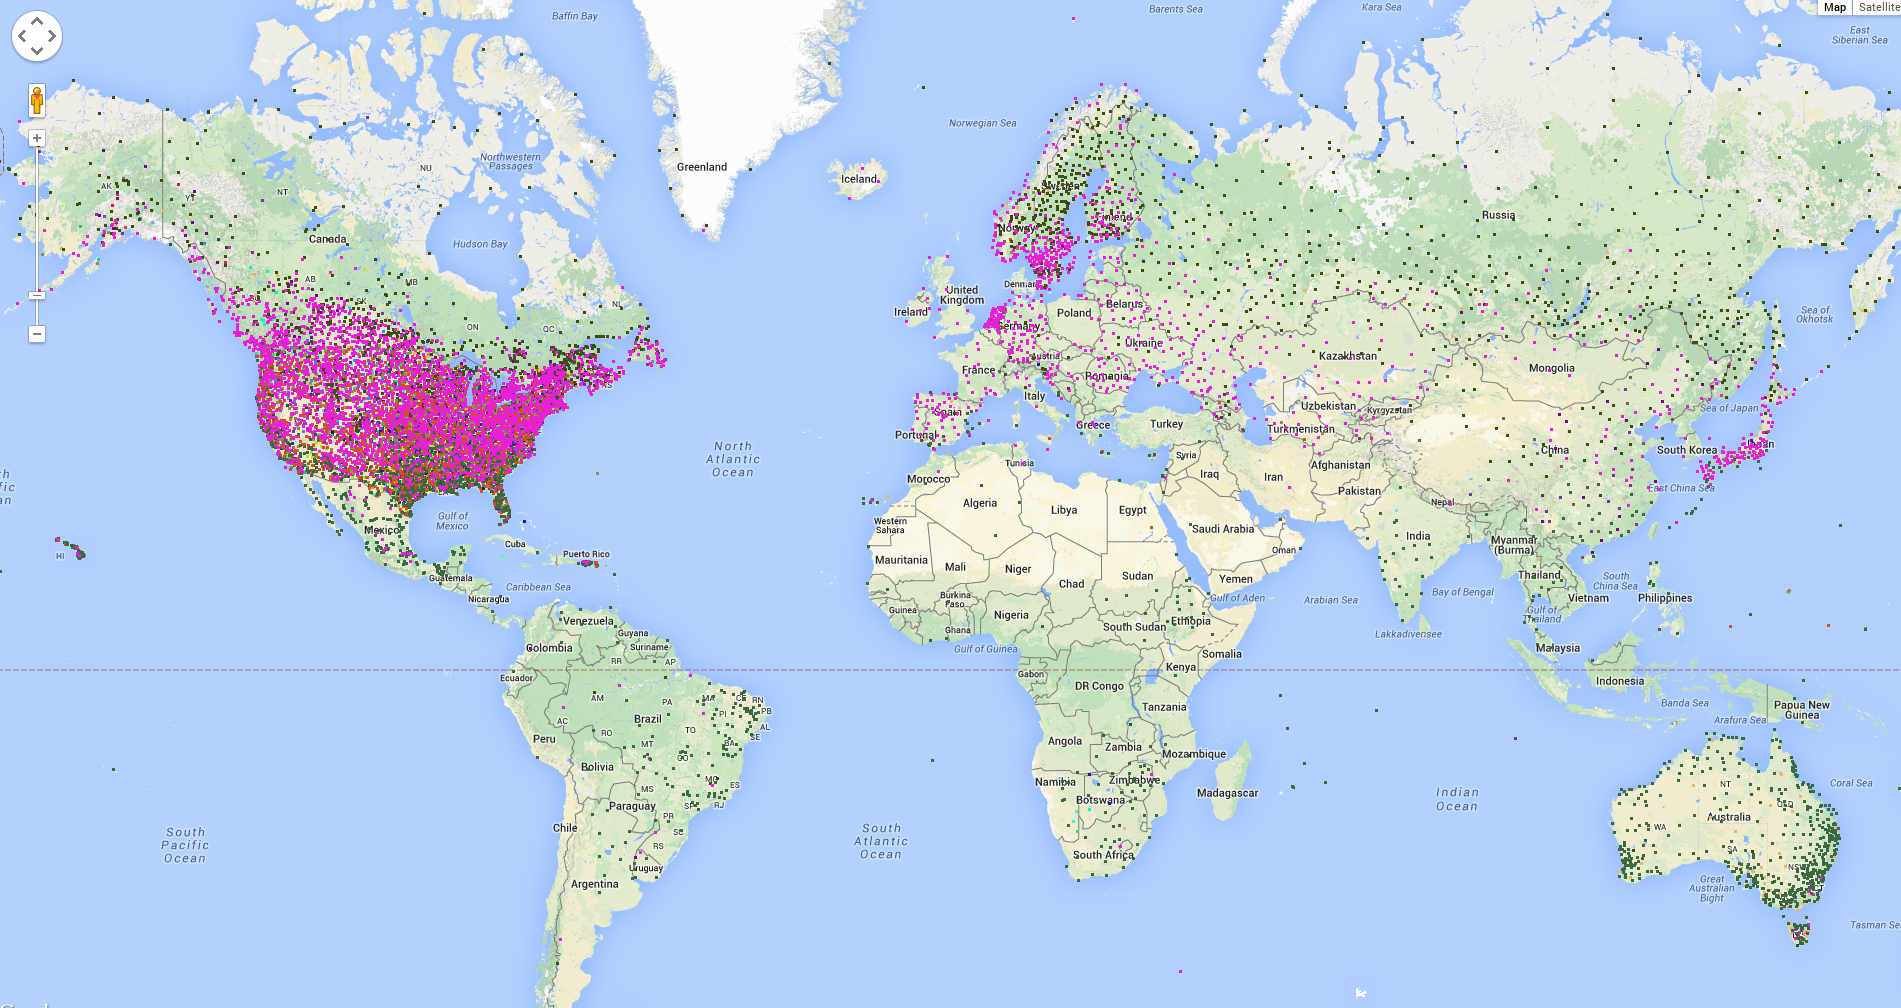
\includegraphics[width =.65\linewidth]{figure/1983.png}\\         1983 \\
        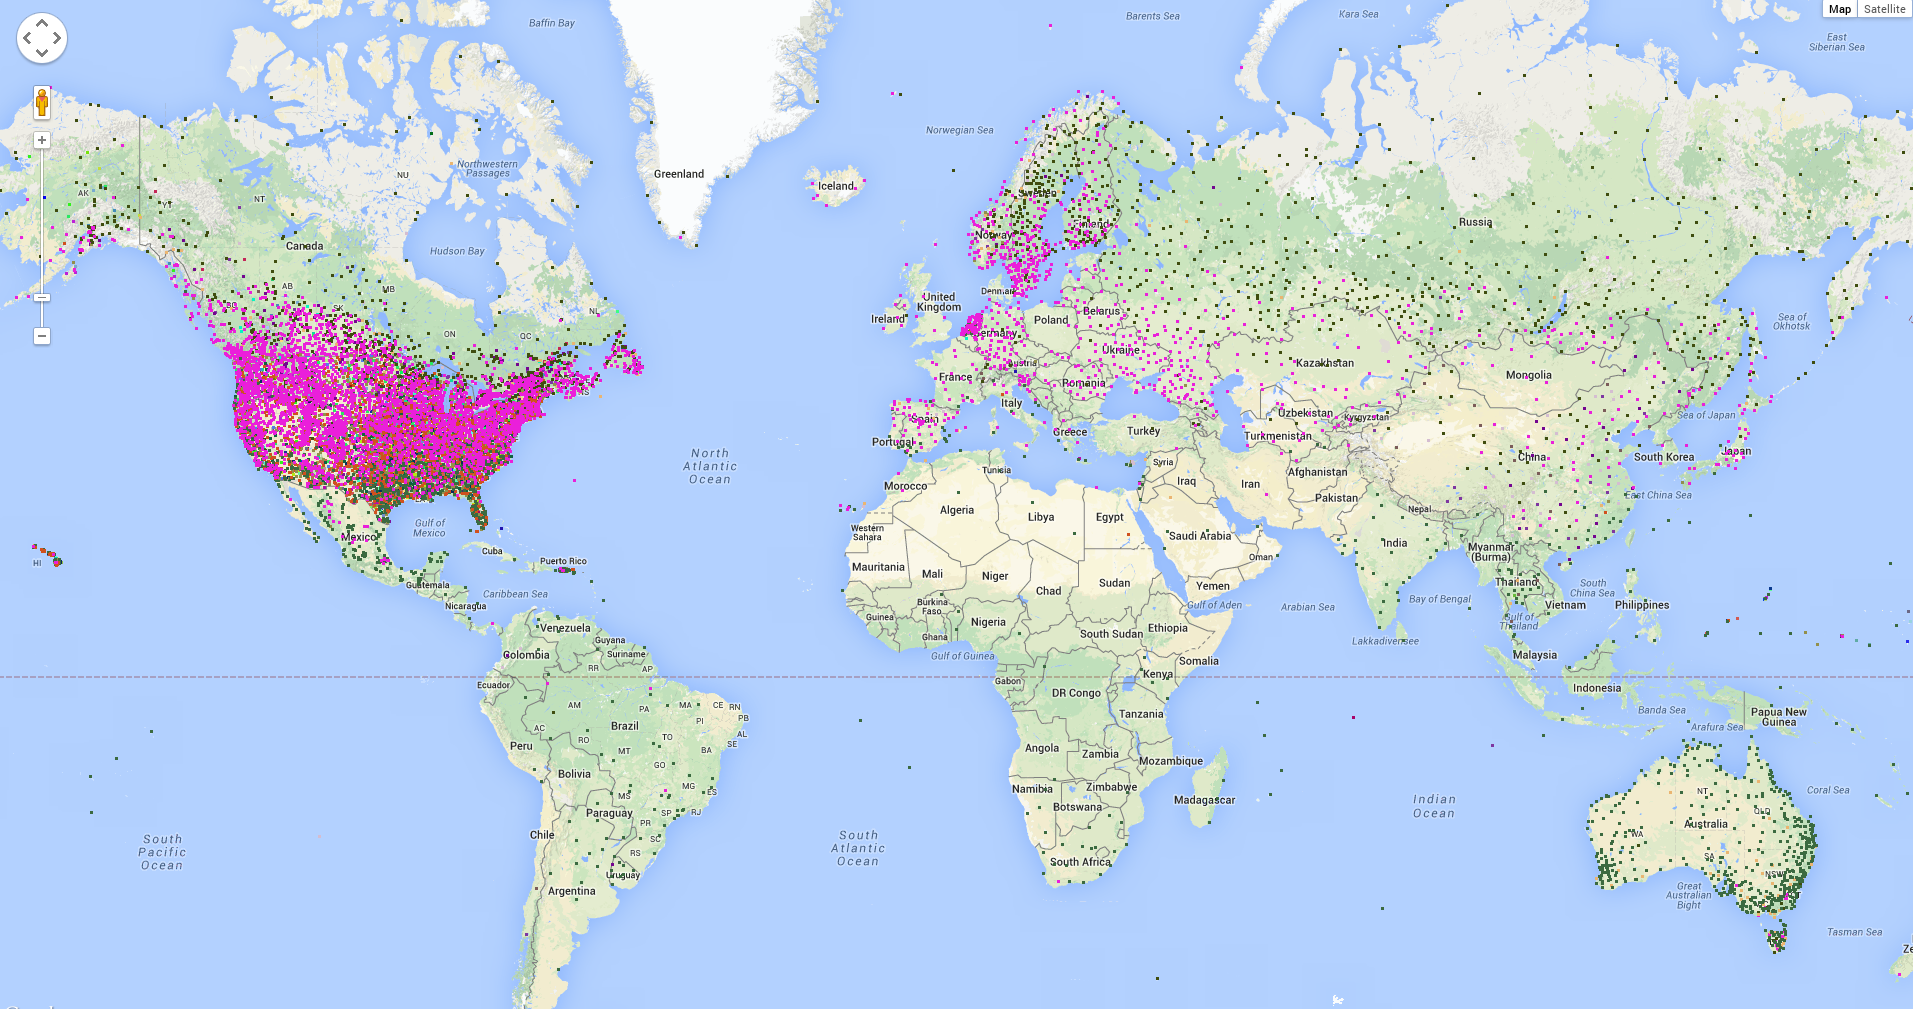
\includegraphics[width =.65\linewidth]{figure/1993.png} \\
        1993 \\
        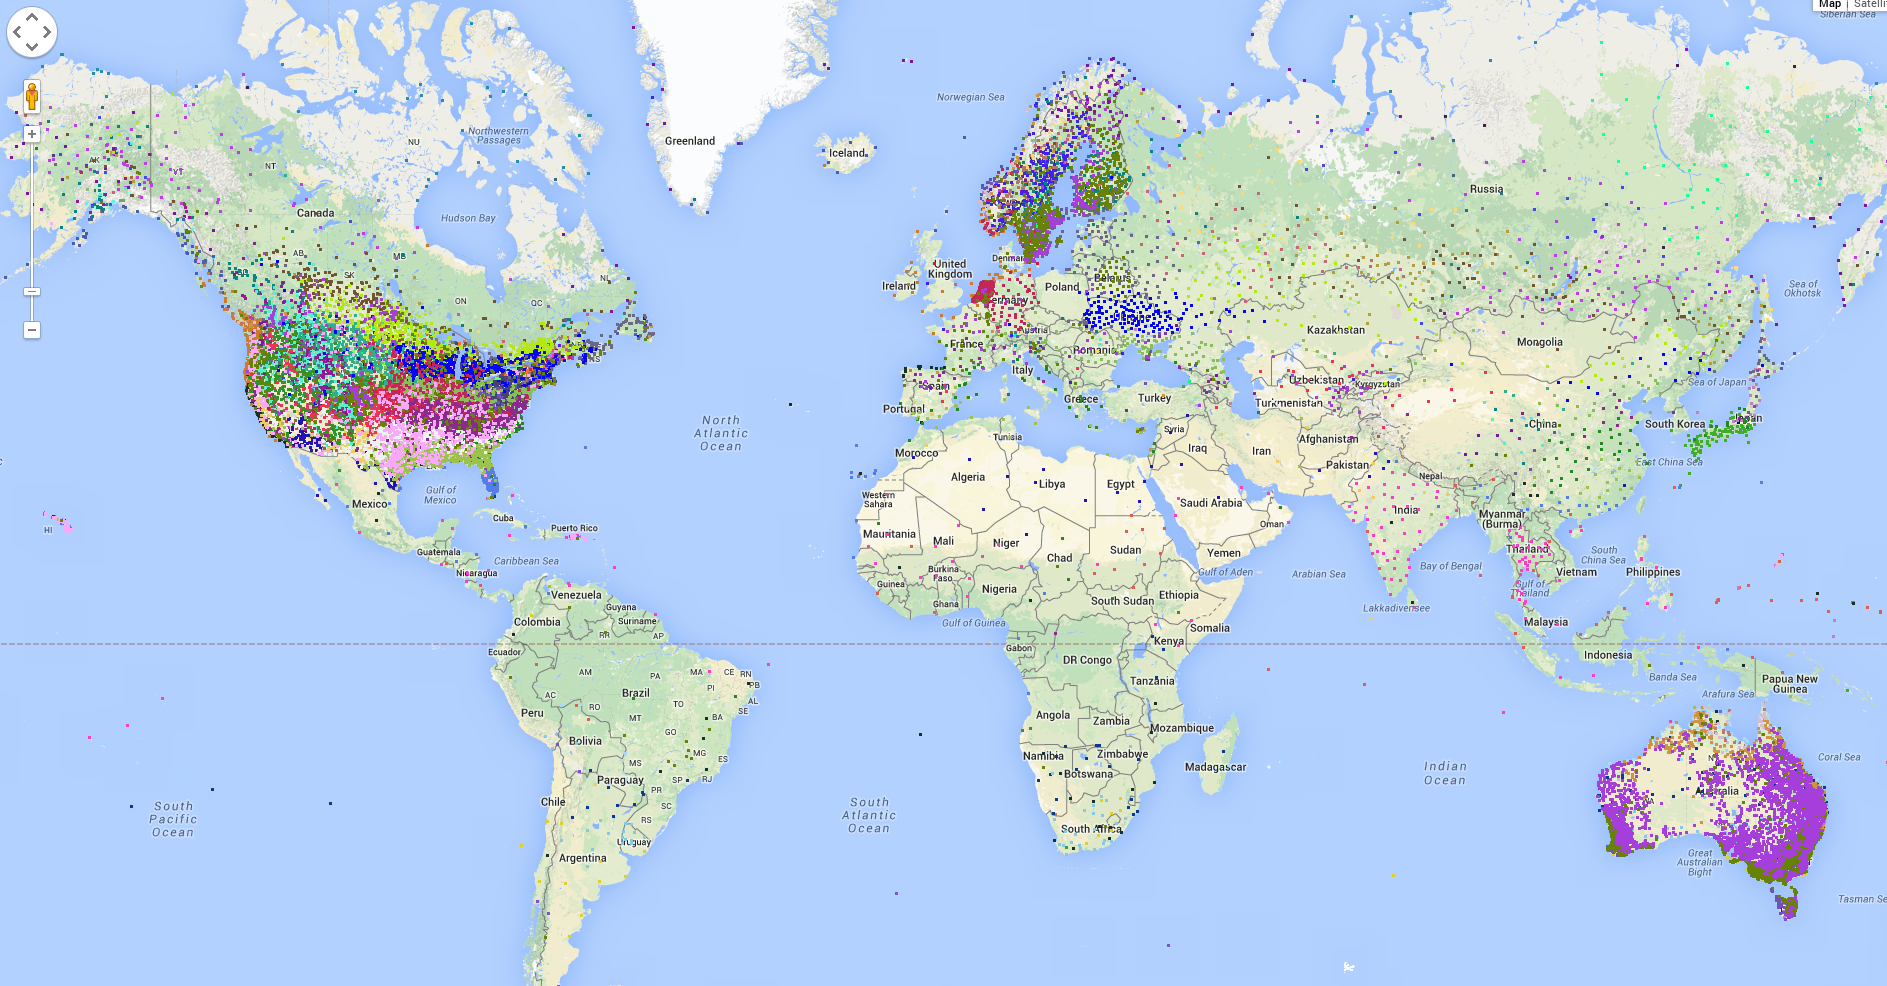
\includegraphics[width =.65\linewidth]{figure/2003.png} \\         2003 \\
        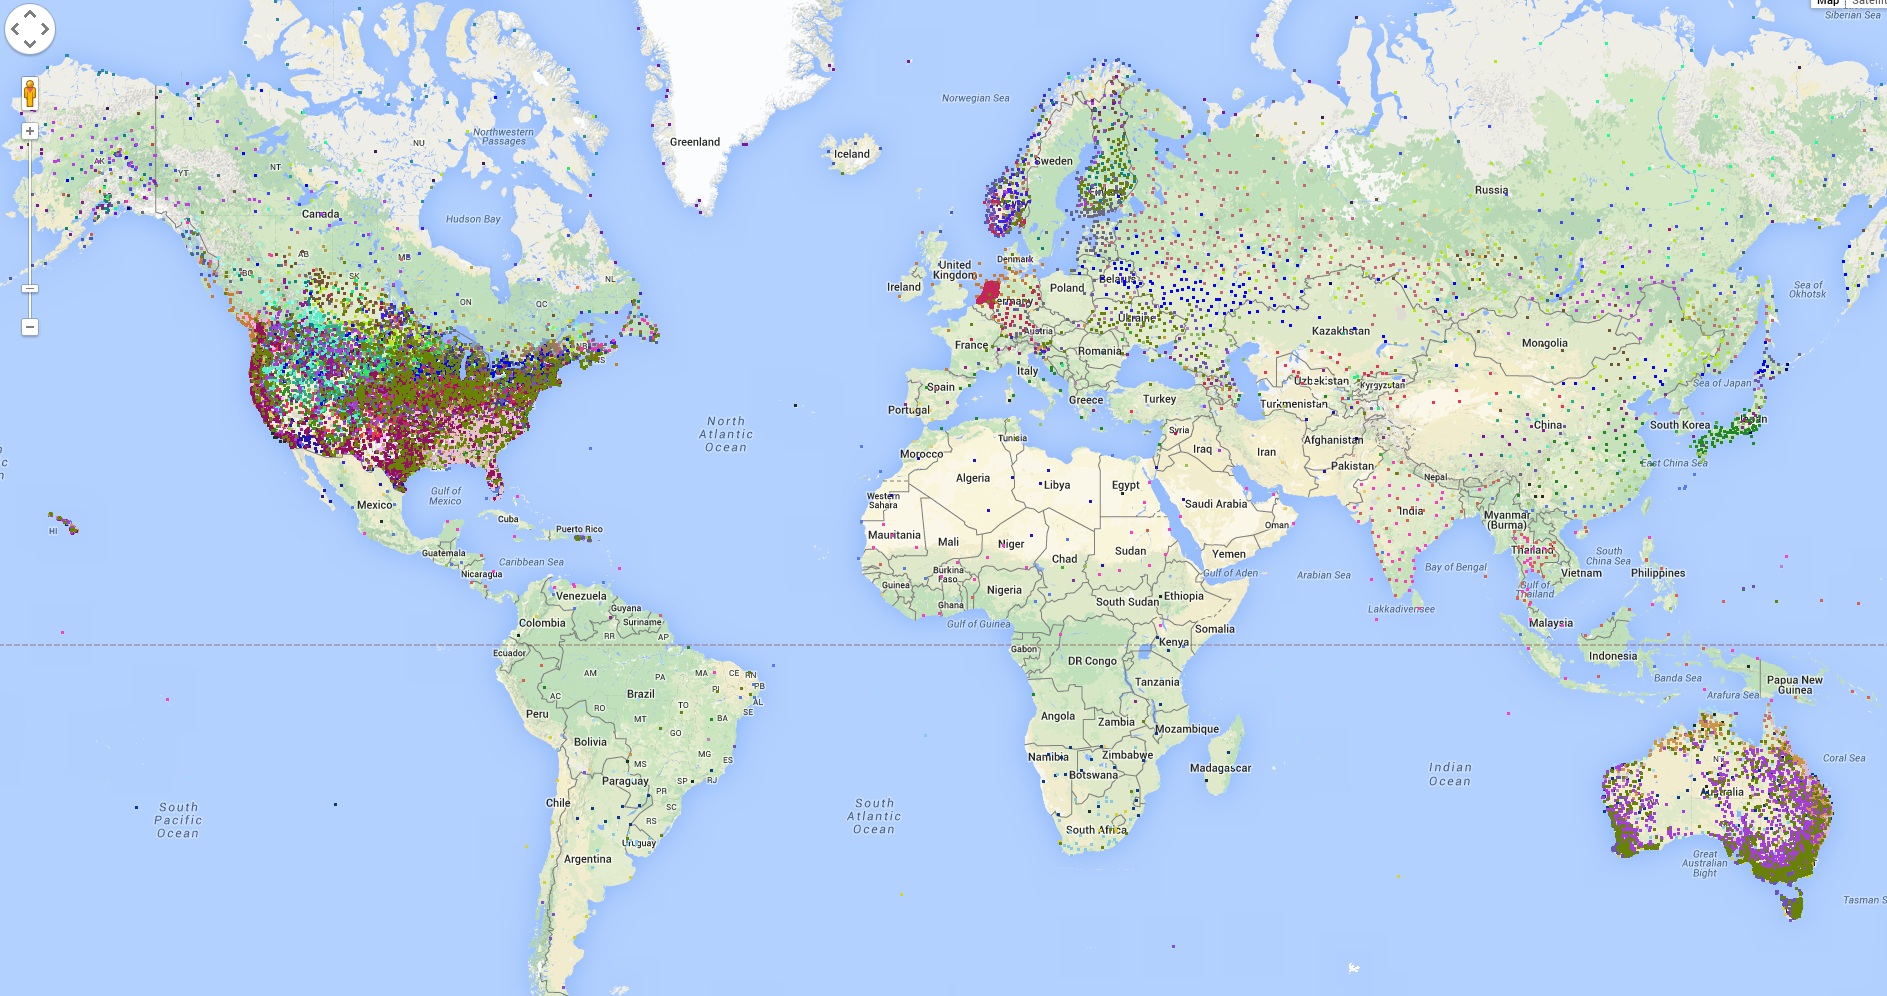
\includegraphics[width =.65\linewidth]{figure/2013.png} \\
        2013\\
    \end{tabular}
    \caption{Clustering results of different years.}
    \label{fig:ClusteringFlow}
\end{figure}

From the clustering flow spanning over 4 decades in Fig \ref{fig:ClusteringFlow}, we are still not satisfied with the current results. In the following, we will discuss a few aspects of the visualization, as well as analysis with possible solutions in the next stage.

From the results, we can see there are only 3 big clusters (Majority of North America, Asia and Russia, Region around Florida) even if we set the number to be 300 for Kmeans. It does not align well with our prior geology knowledge and expected results. There are several possible reasons for this results:

1. We are eliminating data points whose features have relatively large number of missing values. Our threshold might be improper right now. For example, we can observe few points in China while there do exists much more data points in the raw data. It exerts the potential risk of removing possible climate clusters where monitoring data are not complete in all of the five measurements.

2. As we employ uniform sampling to generate coreset, we are still making efforts to analyse 2 specific distributions: (1) distribution of  numbers of data points represented by each coreset point. (2) distribution of numbers of data points represented by each cluster in coreset. If this distribution is close to uniform distribution, it means points in coreset represent unbalanced neighborhood. Then we can conclude our sampling strategy might be improper. We will adjust our sampling strategy and parameters to improve the result quality before the next milestone.

However, there are also some encouraging points in the current results. From the flow from 1983 to 2013, we can observe the three biggest clusters covering roughly the same areas with minor difference. It is a good indication that similar year-wise climate patterns are clustered into the same cluster.

We will make efforts in verifying the correctness of sampling strategy, validity of features and different parameter. We expect better results before the last milestone.

\subsection{Scalability}
For our feature generation tasks, we employ the following EMR master-slave pair for computation. A m3.2xlarge machine with 8 cores and 30GB memory is deployed as the master server, 2 m1.xlarge machines with 4 cores and	15GB memory are employed as slave clients. The running time and peak memory consumption for different feature generation task is summarized in the following table.

\begin{table}[H]
    \begin{tabular}{| c | c | c | c |}
    \hline
    Task & running time & peak memory & normalized instance hour \\
    \hline
    \hline
    Extract feature with missing value & 3h45min & 25GB & 124h\\
    \hline
    Calculate mean and variance of features & 40min & 25GB & 31h\\
    \hline
    Fill missing values and normalize features & 3h47min & 25GB & 124h\\
    %\hline
%    Recalculating mean and variance for normalization &  &  &\\
%    \hline
%    Feature normalization &  &  & \\
    \hline
    \end{tabular}
    \caption{Scalability performance of tasks related to feature generation.}
    \label{tbl:PerfTable}
\end{table}

As we meet difficulties in installing scikit learn library with bootstrap script when launching clusters. We set up Hadoop 2.5.2 environment on a local machine with a quad-core i5-4570 3.2Ghz processor and 16 GB memory. To meet the memory requirement for running intensive tasks, we set up the hadoop mapper and reducer memory at \textit{mapred-site.xml } as the following snippet shows.

\begin{lstlisting}
<configuration>
    <property>
        <name>mapred.job.tracker</name>
        <value>localhost:54311</value>
    </property>
    <property>
        <name>mapreduce.map.memory.mb</name>
        <value>4096</value>
    </property>
    <property>
        <name>mapreduce.reduce.memory.mb</name>
        <value>8192</value>
    </property>
    <property>
        <name>mapreduce.map.java.opts</name>
        <value>-Xmx3072m</value>
    </property>
    <property>
        <name>mapreduce.reduce.java.opts</name>
        <value>-Xmx6144m</value>
    </property>
</configuration>

\end{lstlisting}


%\bibliographystyle{plain}
%\bibliography{Proposal}

\end{document}
